\documentclass[11pt,a4paper]{article}
\usepackage[margin=0.78in]{geometry}
\usepackage[T1]{fontenc}
\usepackage[utf8]{inputenc}
\usepackage{lmodern}
\usepackage{amsmath,amssymb}
\usepackage{booktabs}
\usepackage{array}
\usepackage{float}
\usepackage{xcolor}
\usepackage{tikz}
\usetikzlibrary{arrows.meta,positioning,calc,fit,shadows.blur}
\usepackage{hyperref}
\usepackage{caption}
\usepackage{graphicx}
\usepackage{subcaption}
\usepackage{enumitem}
\usepackage[numbers,square]{natbib}
\usepackage{seqsplit}
% Long hex digests (a sha256 and a git commit) have no break points and would otherwise
% run into the margin. \hex lets them wrap anywhere, which is correct for a digest.
\newcommand{\hex}[1]{\texttt{\seqsplit{#1}}}

\definecolor{navy}{HTML}{24496B}
\definecolor{bluefill}{HTML}{E8F1FA}
\definecolor{green}{HTML}{2F855A}
\definecolor{greenfill}{HTML}{E8F5ED}
\definecolor{orange}{HTML}{C56A16}
\definecolor{orangefill}{HTML}{FFF0DF}
\definecolor{purple}{HTML}{7057B7}
\definecolor{purplefill}{HTML}{EFEAFB}
\definecolor{red}{HTML}{B94A48}
\definecolor{redfill}{HTML}{FCE8E8}
\definecolor{grayline}{HTML}{B8C2CC}
\definecolor{grayfill}{HTML}{F5F7F9}
\definecolor{darkgray}{HTML}{3A4651}

\hypersetup{colorlinks=true,linkcolor=navy,urlcolor=navy,citecolor=navy}

\tikzset{
  card/.style={draw=grayline, rounded corners=3pt, line width=.8pt,
               minimum width=32mm, minimum height=10mm, align=center,
               font=\small, inner sep=4pt, fill=white},
  shared/.style={card, draw=navy!55, fill=bluefill},
  base/.style={card, draw=green!70, fill=greenfill},
  plm/.style={card, draw=orange!80, fill=orangefill},
  struct/.style={card, draw=purple!75, fill=purplefill},
  bad/.style={card, draw=red!70, fill=redfill},
  data/.style={card, draw=navy!55, fill=bluefill, minimum width=38mm},
  arrow/.style={-{Latex[length=2.6mm]}, line width=.9pt, draw=darkgray},
  thinarr/.style={-{Latex[length=2.2mm]}, line width=.7pt, draw=darkgray},
  xarr/.style={-{Latex[length=2.2mm]}, line width=.7pt, draw=red!70, dashed},
  lbl/.style={font=\footnotesize, text=darkgray, align=center}
}

\newcommand{\rhop}{\rho_{\text{pool}}}
\newcommand{\rhow}{\rho_{\text{within}}}

\title{\vspace{-1.6em}\textbf{Can foundation models improve peptide--HLA stability prediction?}\\
\large A leakage-controlled negative result, and what it costs to establish}
\author{Serova Protein Engineering Track (Track 3) \\ London AI $\times$ Science Hackathon, 3--4 October 2026}
\date{}

\begin{document}
\maketitle
\vspace{-2.2em}

\begin{abstract}
\noindent
We ask whether pretrained protein language models improve prediction of peptide--HLA class~I
kinetic stability. On a leakage-controlled split of 28{,}166 measured half-lives, the answer is
\textbf{no}: a one-hot multilayer perceptron over the peptide and the NetMHCpan pseudosequence
reaches $\rhop = 0.780$ on validation and $0.806$ on a test split read exactly once, and
\textbf{no foundation-model configuration we tested matches it}. The negative survives every
obvious objection --- encoder depth, an 80$\times$ scale sweep, LoRA fine-tuning, cross-chain
attention, label budget, and three further model families including a published peptide--MHC
model. We go further than the negative and explain it: ESM-2's notion of which residues matter is
\emph{orthogonal} to this endpoint (rank correlation $-0.03$ against the trained model's ablation
profile); predicted structures are \emph{correct} yet their geometry does not track half-life
(Mantel $r=-0.111$ at 92\% power for $r=0.2$); and two unrelated routes to modelling the
peptide--groove interaction --- pretraining on 96M protein--protein interactions, or a
561{,}793-parameter attention head --- buy the \emph{same} $+0.16$ and both stop below the
baseline. We report prediction intervals whose marginal coverage holds (90.5\% at a 90\% target)
and whose per-allele coverage does not (68.8\% to 100\%), the empirical ceiling the task permits
($\approx 0.823$), and the compute bill (7.5 GPU-hours, \$15.26), of which 88\% was spent on
configurations that land inside seed noise or below a free baseline.
\end{abstract}

\section{Problem setup and notation}

Each record pairs an HLA class~I groove sequence $m$ with a peptide $p$ and an experimentally
measured complex half-life $t_{1/2}$ in hours. Models predict the log-transformed target
\[
y=\log\!\left(1+t_{1/2}\right),\qquad \hat t_{1/2}=\exp(\hat y)-1,
\]
which is used because the raw distribution spans $0$ to $256.7$~h with a median of $1.1$~h and a
point mass of $5{,}679$ exact zeros (20.2\% of rows).

Notation is fixed for the whole report.

\begin{table}[H]
\centering\small
\begin{tabular}{@{}llp{86mm}@{}}
\toprule
\textbf{Symbol} & \textbf{Domain} & \textbf{Meaning} \\
\midrule
$p$ & $\Sigma^{9}$ & peptide, 9-mer over the 20-letter amino-acid alphabet $\Sigma$ \\
$m$ & $\Sigma^{182}$ & HLA class~I $\alpha_1\alpha_2$ groove domain \\
$\pi(m)$ & $\Sigma^{34}$ & NetMHCpan pseudosequence: the 34 crystallographic contact positions \\
$a$ & $\{1,\dots,75\}$ & allele identity, as a categorical label \\
$t_{1/2}$ & $[0,256.7]$ & measured half-life, hours \\
$y$ & $\mathbb{R}_{\ge 0}$ & $\log(1+t_{1/2})$, the regression target \\
$c(p)$ & $\{1,\dots,5410\}$ & peptide cluster id under Hamming distance $\le 2$ \\
$E_\theta$ & $\Sigma^{L}\!\to\!\mathbb{R}^{L\times d}$ & frozen encoder producing per-residue states \\
$d$ & $\mathbb{N}$ & encoder width (320, 480, 640, 1280 across models tested) \\
$\rhop$ & $[-1,1]$ & Spearman correlation over all rows pooled \\
$\rhow$ & $[-1,1]$ & mean Spearman inside each allele with $\ge 12$ rows \\
\bottomrule
\end{tabular}
\caption{Notation. $\rhow$ is the primary metric; Section~\ref{sec:eval} explains why.}
\end{table}

\section{Data and the leakage-controlled split}

\subsection{Why a row split is wrong here}

94\% of peptides in this dataset are measured against more than one allele. A random split over
\emph{rows} therefore places the same peptide on both sides of the partition, and a model can
score well by recognising the fragment rather than by modelling the interaction. Grouping by
\emph{exact} peptide removes that, but not the weaker form: a 9-mer differing by one substitution
is 89\% identical, and the field's common 80\%-identity convention admits exactly such pairs.

We therefore cluster peptides at \textbf{Hamming distance $\le 2$} by single-linkage and assign
whole clusters, which is strictly more conservative than both alternatives.

\begin{figure}[H]
\centering
\resizebox{0.95\textwidth}{!}{%
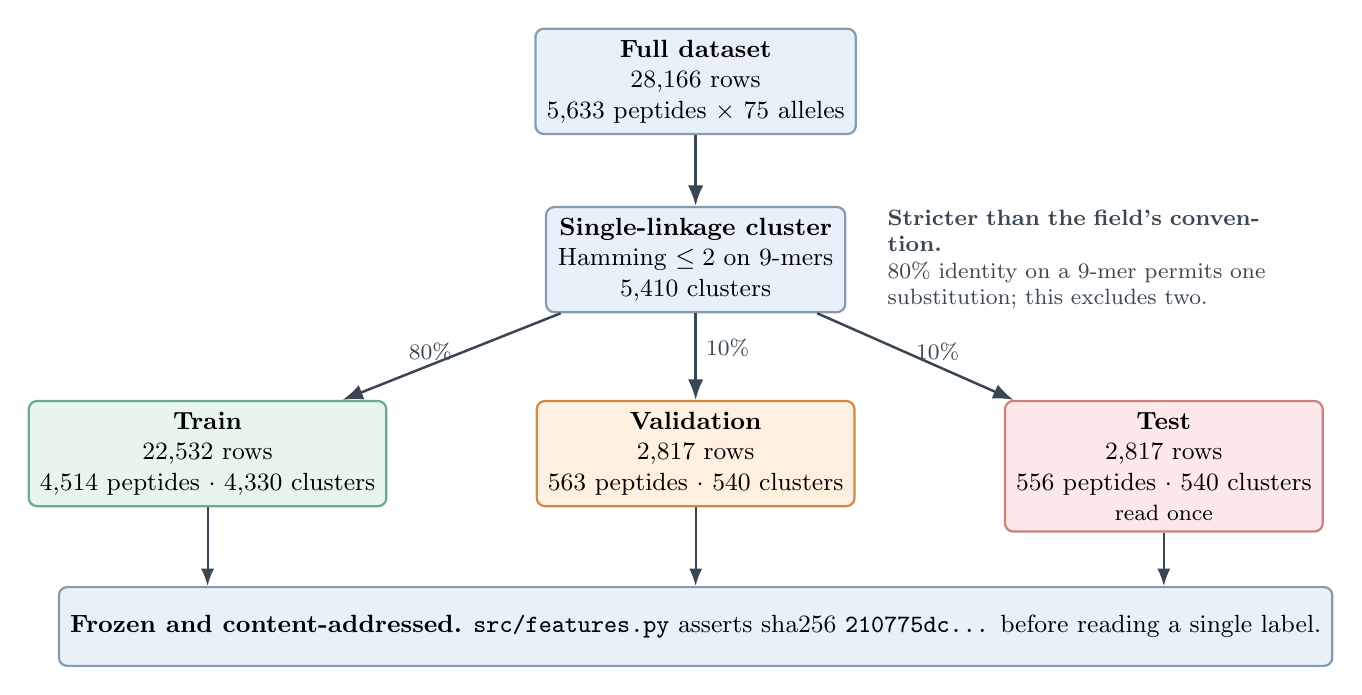
\begin{tikzpicture}[node distance=9mm and 12mm]
  \node[data] (full) {\textbf{Full dataset}\\28,166 rows\\5,633 peptides $\times$ 75 alleles};
  \node[data, below=9mm of full] (cl) {\textbf{Single-linkage cluster}\\Hamming $\le 2$ on 9-mers\\5,410 clusters};
  \node[lbl, right=4mm of cl, text width=52mm, align=left]
    {\textbf{Stricter than the field's convention.}\\80\% identity on a 9-mer permits one
     substitution; this excludes two.};

  \node[base, below left=11mm and 20mm of cl, minimum width=42mm] (tr)
       {\textbf{Train}\\22,532 rows\\4,514 peptides $\cdot$ 4,330 clusters};
  \node[plm, below=11mm of cl, minimum width=36mm] (va)
       {\textbf{Validation}\\2,817 rows\\563 peptides $\cdot$ 540 clusters};
  \node[bad, below right=11mm and 20mm of cl, minimum width=36mm] (te)
       {\textbf{Test}\\2,817 rows\\556 peptides $\cdot$ 540 clusters\\\footnotesize read once};

  \node[shared, below=10mm of va, minimum width=120mm] (guard)
       {\textbf{Frozen and content-addressed.} \texttt{src/features.py} asserts
        sha256 \texttt{210775dc\ldots} before reading a single label.};

  \draw[arrow] (full) -- (cl);
  \draw[arrow] (cl) -- node[lbl,left,pos=.45] {80\%} (tr);
  \draw[arrow] (cl) -- node[lbl,right,pos=.4] {10\%} (va);
  \draw[arrow] (cl) -- node[lbl,right,pos=.45] {10\%} (te);
  % straight down onto the guard's top edge; an |- route would cross the box and strike its text
  \draw[thinarr] (tr.south) -- (tr.south |- guard.north);
  \draw[thinarr] (va.south) -- (va.south |- guard.north);
  \draw[thinarr] (te.south) -- (te.south |- guard.north);
\end{tikzpicture}}
\caption{The leakage-controlled split. Whole clusters are assigned, so no peptide in one partition
is within two substitutions of any peptide in another. The hash guard means a job that somehow
receives a different split fails immediately rather than quietly reporting a number against other
data.}
\label{fig:split}
\end{figure}

\subsection{The split was validated, not assumed}

Two checks run against the frozen assignments. First, a \textbf{boundary probe}: a synthetic
peptide 2 edits from a training peptide must be detected as a near-duplicate, and one at 3 edits,
verified clear of \emph{every} training peptide, must not be. Both behave correctly, which
establishes the detector separates rather than merely firing. Second, measured
\textbf{cross-allele agreement decays monotonically with pseudosequence distance} --- $0.823$,
$0.659$, $0.474$, $0.318$ at Hamming $1,2,3,4$ --- with no model involved, confirming that
sequence distance carries the biological signal the split assumes it does.

\section{Evaluation protocol}
\label{sec:eval}

\subsection{A floor, not zero}

A per-allele median containing \textbf{no peptide information whatsoever} scores
$\rhop = 0.563$. Every pooled figure in this field must be read against that number rather than
against zero, because pooled Spearman rewards a model merely for knowing which allele it is
looking at. This is not a small correction: it is 72\% of the way from zero to our best model.

\subsection{Within-allele Spearman is primary}

$\rhow$ averages the Spearman correlation computed \emph{inside} each allele with at least 12
rows. It is the metric that cannot be inflated by across-allele structure, and it is also the
clinical question --- ranking one patient's candidate peptides within the allele they actually
carry. Section~\ref{sec:metric} gives a case where the two metrics disagree so sharply that the
choice decides whether a model appears useless or useful.

\subsection{Intervals from a cluster bootstrap}

All confidence intervals come from 2{,}000 paired bootstrap draws (seed 2026) resampling the
\textbf{540 validation peptide clusters}, never rows. Rows inside one cluster are within two
substitutions and are not independent; resampling them would claim precision we have not earned.

\subsection{A negative control that found something}

Shuffling training labels scored $+0.104$, which looks like leakage. It is not. A fixed-epoch
rerun scored $+0.02$, isolating the remaining $+0.08$ as \textbf{epoch-selection optimism}: the
act of choosing the best epoch against validation inflates every validation figure by roughly
that much. Paired differences cancel it, which retroactively justifies reporting comparisons
rather than absolute values.

\subsection{Test discipline}

The test split was read \textbf{once}, after 21 runs had frozen every architecture, budget and
selection rule. A guard file in \texttt{src/test\_evaluation.py} refuses a second read. One model
(L150) was deliberately omitted from that read because scoring it would have required retraining
\emph{after} seeing the test table; it was closed later by keeping the validation-selected
checkpoint and scoring inside the same run (Section~\ref{sec:results}).

\section{Models}

\subsection{The ladder}

\begin{figure}[H]
\centering
\resizebox{0.97\textwidth}{!}{%
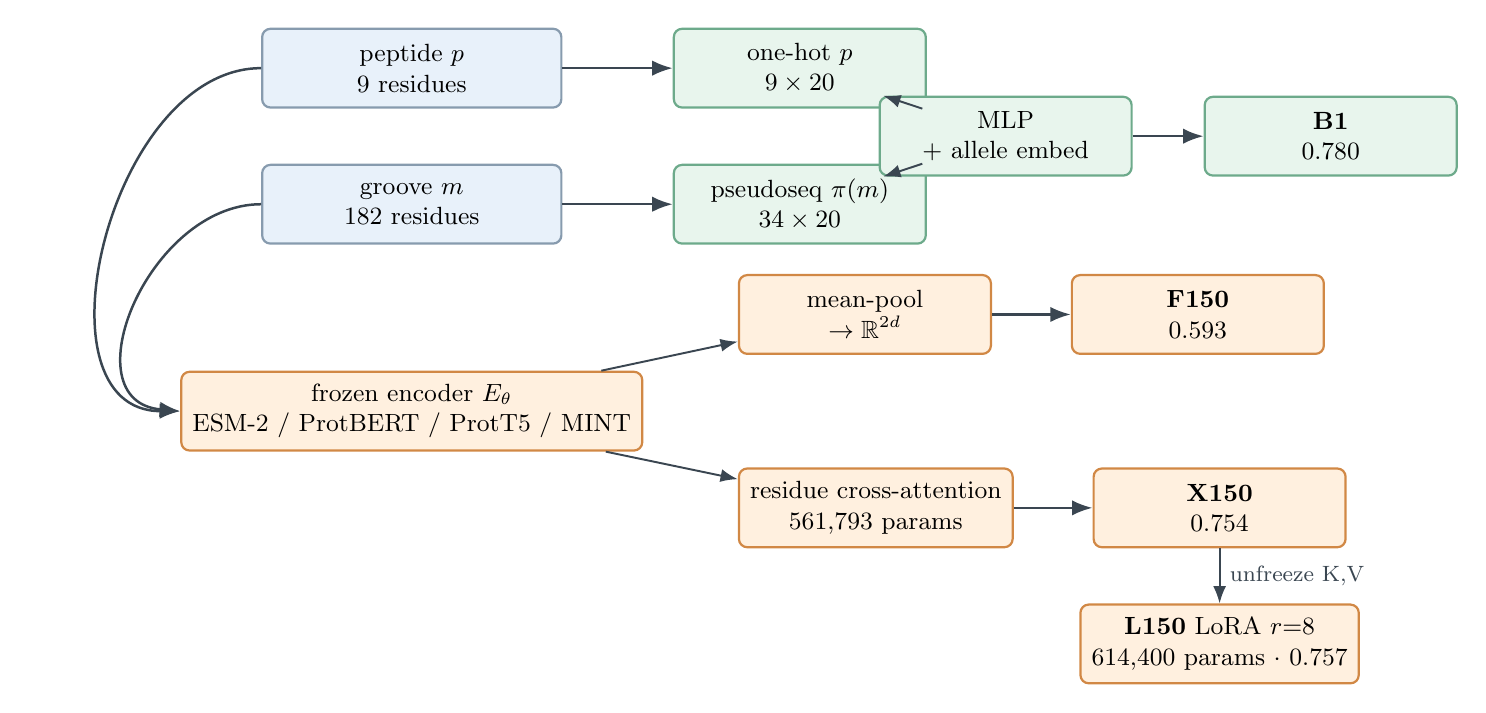
\begin{tikzpicture}[node distance=7mm and 9mm]
  \node[data] (pep) {peptide $p$\\$9$ residues};
  \node[data, below=7mm of pep] (hla) {groove $m$\\$182$ residues};

  % baseline path
  \node[base, right=14mm of pep] (oh) {one-hot $p$\\$9\times20$};
  \node[base, right=14mm of hla] (ps) {pseudoseq $\pi(m)$\\$34\times20$};
  \node[base, right=10mm of $(oh)!0.5!(ps)$] (mlp) {MLP\\+ allele embed};
  \node[base, right=9mm of mlp] (b1) {\textbf{B1}\\$0.780$};

  % PLM path
  \node[plm, below=16mm of hla] (enc) {frozen encoder $E_\theta$\\ESM-2 / ProtBERT / ProtT5 / MINT};
  \node[plm, above right=2mm and 12mm of enc] (pool) {mean-pool\\$\to \mathbb{R}^{2d}$};
  \node[plm, below right=2mm and 12mm of enc] (xatt) {residue cross-attention\\$561{,}793$ params};
  \node[plm, right=10mm of pool] (f150) {\textbf{F150}\\$0.593$};
  \node[plm, right=10mm of xatt] (x150) {\textbf{X150}\\$0.754$};
  \node[plm, below=7mm of x150] (l150) {\textbf{L150} LoRA $r{=}8$\\$614{,}400$ params $\cdot$ $0.757$};

  \draw[arrow] (pep) -- (oh);
  \draw[arrow] (hla) -- (ps);
  \draw[thinarr] (oh) -- (mlp);
  \draw[thinarr] (ps) -- (mlp);
  \draw[arrow] (mlp) -- (b1);
  \draw[arrow] (pep.west) to[out=180,in=180,looseness=1.1] (enc.west);
  \draw[arrow] (hla.west) to[out=180,in=175,looseness=1.3] (enc.west);
  \draw[thinarr] (enc) -- (pool);
  \draw[thinarr] (enc) -- (xatt);
  \draw[arrow] (pool) -- (f150);
  \draw[arrow] (xatt) -- (x150);
  \draw[thinarr] (x150) -- node[lbl,right] {unfreeze K,V} (l150);
\end{tikzpicture}}
\caption{The two paths. Everything below the encoder is a protein language model; the top path has
none and wins. Figures are validation $\rhop$.}
\label{fig:arch}
\end{figure}

\subsection{What each rung isolates}

\begin{table}[H]
\centering\small
\begin{tabular}{@{}llp{74mm}@{}}
\toprule
\textbf{Rung} & \textbf{Trainable} & \textbf{The single question it answers} \\
\midrule
B0b & --- & How much of pooled $\rho$ is available with \emph{no} peptide information? \\
B1$'$ & MLP & Does a one-hot allele \emph{label} suffice, without its sequence? \\
B1 & MLP & Does the crystallography-derived pseudosequence add over the label? \\
F150 & head & What does a frozen PLM give when position is destroyed by pooling? \\
X150 & $561{,}793$ & What does the \emph{head} contribute on identical frozen embeddings? \\
L150 & $614{,}400$ & Does adapting the encoder itself (LoRA on K,V of all 30 layers) help? \\
\bottomrule
\end{tabular}
\caption{Each rung changes exactly one thing from the rung above it.}
\end{table}

LoRA uses the standard reparameterisation \citep{hu2022lora}
\(W_{\text{eff}} = W + \tfrac{\alpha}{r}BA\) with $r=8$, $\alpha=16$, dropout $0.05$, applied to
the key and value projections of all 30 layers: 60 modules, $614{,}400$ parameters, 0.41\% of the
backbone.

\subsection{Fair comparison across encoders}

Every encoder --- ESM-2 at four sizes \citep{lin2023esm2}, ProtBERT and ProtT5
\citep{elnaggar2021prottrans}, and MINT \citep{ullanat2026mint} --- is run through the
\textbf{identical} head, split, three seeds, early-stopping budget (40 epochs, patience 6), and a
two-learning-rate choice ($10^{-3}$, $3\times10^{-4}$) with the better kept. Only the encoder
changes. This matters: an early version of our scale sweep gave ESM-2 650M a single learning rate
and recorded $0.526$, \emph{below the no-peptide floor}. That was a convergence failure, not a
finding; the fair two-rate protocol gives $0.764$.

\section{Compute setup and dataflow}

\begin{figure}[H]
\centering
\resizebox{0.93\textwidth}{!}{%
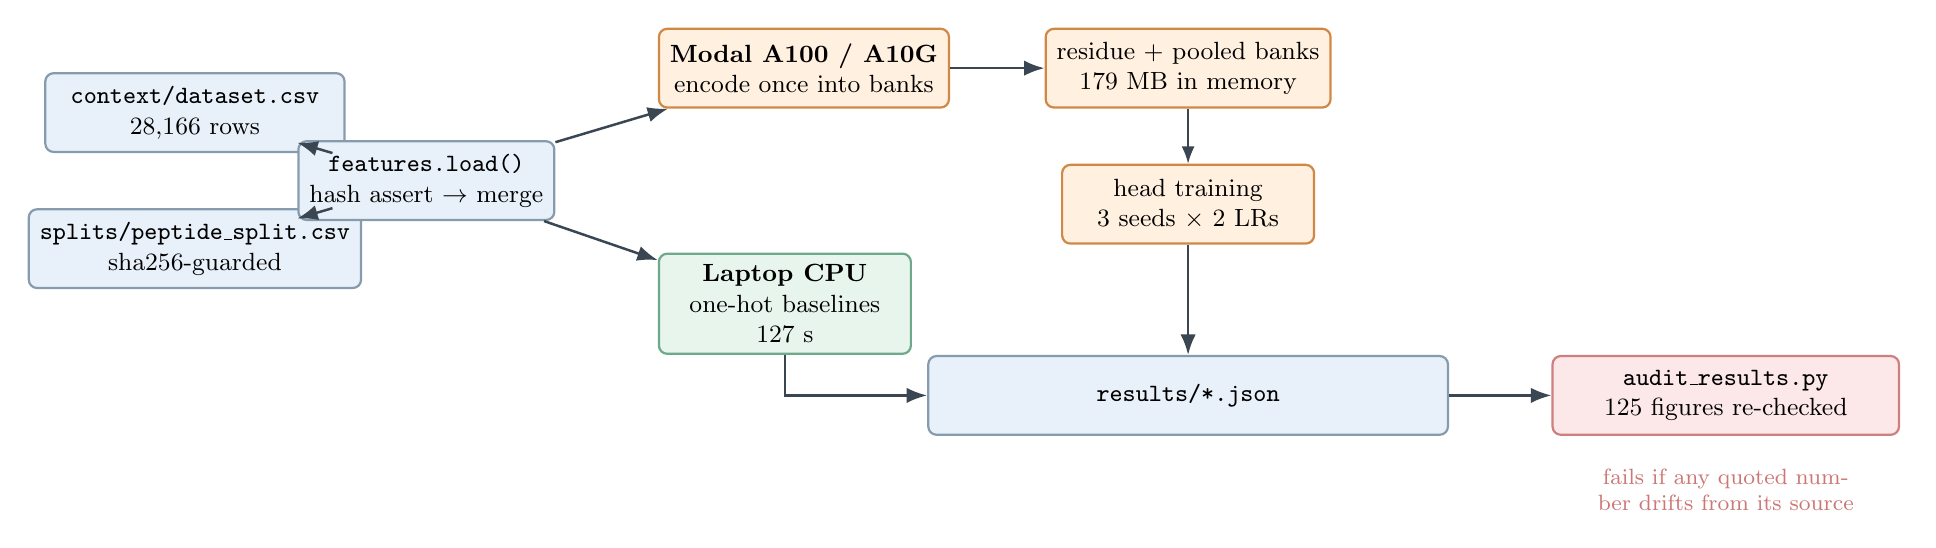
\begin{tikzpicture}[node distance=8mm and 11mm]
  \node[data] (csv) {\texttt{context/dataset.csv}\\28,166 rows};
  \node[data, below=7mm of csv] (split) {\texttt{splits/peptide\_split.csv}\\sha256-guarded};
  \node[shared, right=13mm of $(csv)!0.5!(split)$] (feat) {\texttt{features.load()}\\hash assert $\to$ merge};

  \node[plm, above right=4mm and 13mm of feat] (gpu) {\textbf{Modal A100 / A10G}\\encode once into banks};
  \node[plm, right=12mm of gpu] (bank) {residue + pooled banks\\$179$~MB in memory};
  \node[plm, below=7mm of bank] (head) {head training\\3 seeds $\times$ 2 LRs};

  \node[base, below right=4mm and 13mm of feat] (cpu) {\textbf{Laptop CPU}\\one-hot baselines\\127 s};

  \node[shared, below=14mm of head, minimum width=66mm] (res) {\texttt{results/*.json}};
  \node[bad, right=13mm of res, minimum width=44mm] (audit)
       {\texttt{audit\_results.py}\\125 figures re-checked};
  \node[lbl, below=3mm of audit, text width=44mm, text=red!75]
       {fails if any quoted number drifts from its source};

  \draw[arrow] (csv) -- (feat);
  \draw[arrow] (split) -- (feat);
  \draw[arrow] (feat) -- (gpu);
  \draw[arrow] (feat) -- (cpu);
  \draw[arrow] (gpu) -- (bank);
  \draw[thinarr] (bank) -- (head);
  \draw[arrow] (head) -- (res);
  \draw[arrow] (cpu) |- (res);
  \draw[arrow] (res) -- (audit);
\end{tikzpicture}}
\caption{Dataflow. Encoding happens once into shared banks indexed per row; materialising
per-row tensors instead would have required 10.5~GB, where the banks occupy a measured 179~MB.}
\label{fig:flow}
\end{figure}

\section{Results}
\label{sec:results}

\subsection{The ladder}

\begin{table}[H]
\centering\small
\resizebox{\textwidth}{!}{%
\begin{tabular}{@{}lccc@{}}
\toprule
\textbf{Rung} & $\rhop$ \textbf{[95\% CI]} & $\rhow$ \textbf{[95\% CI]} & \textbf{PLM?} \\
\midrule
B0b per-allele median (no peptide info) & 0.563 [0.522, 0.598] & undefined & no \\
F150 frozen ESM-2 150M, mean-pooled & 0.593 [0.556, 0.625] & 0.278 [0.222, 0.320] & yes \\
ProtT5-XL encoder, 1{,}208M & 0.729$^\dagger$ & 0.511$^\dagger$ & yes \\
ProtBERT, 420M & 0.729$^\dagger$ & 0.529$^\dagger$ & yes \\
MINT Stage-1, 814M, mean-pooled & 0.749$^\dagger$ & 0.528$^\dagger$ & yes \\
B1$'$ one-hot peptide + allele identity & 0.748 [0.719, 0.775] & 0.557 [0.508, 0.585] & no \\
X150 frozen ESM-2 150M, cross-attention & 0.754 [0.727, 0.777] & 0.558 [0.508, 0.585] & yes \\
L150 ESM-2 150M, LoRA-adapted & 0.757 [0.732, 0.780] & 0.572 [0.524, 0.599] & yes \\
ESM-2 650M, fair two-LR protocol & 0.764$^\dagger$ & --- & yes \\
\textbf{B1 one-hot + pseudosequence + allele} & \textbf{0.780 [0.756, 0.802]} & \textbf{0.633 [0.588, 0.654]} & \textbf{no} \\
\bottomrule
\end{tabular}}
\caption{Validation. $^\dagger$ not bootstrapped; worst per-seed spread across those rows is
0.039. $\text{B1}-\text{L150} = +0.023\,[+0.007,+0.039]$ pooled and
$+0.060\,[+0.027,+0.094]$ within-allele; both exclude zero.}
\label{tab:ladder}
\end{table}

\subsection{Held-out test, read once}

\begin{table}[H]
\centering\small
\begin{tabular}{@{}lcc@{}}
\toprule
\textbf{Rung} & \textbf{test} $\rhop$ & \textbf{test} $\rhow$ \\
\midrule
B0b per-allele median & 0.573 & undefined \\
F150 frozen ESM-2, mean-pooled & 0.606 & 0.244 \\
X150 frozen ESM-2, cross-attention & 0.756 & 0.535 \\
L150 LoRA-adapted ESM-2 & 0.758 & 0.525 \\
B1$'$ one-hot + allele identity & 0.767 & 0.566 \\
\textbf{B1 one-hot + pseudosequence + allele} & \textbf{0.806} & \textbf{0.645} \\
\bottomrule
\end{tabular}
\caption{Every ordering survives and the gap \emph{widens}. $\text{B1}-\text{X150}$ is $+0.050$
pooled on test against $+0.026$ on validation; $\text{B1}-\text{L150}$ is $+0.048$ and $+0.120$,
roughly double its validation value.}
\label{tab:test}
\end{table}

\subsection{Every obvious objection, tested}

\begin{table}[H]
\centering\small
\resizebox{\textwidth}{!}{%
\begin{tabular}{@{}lll@{}}
\toprule
\textbf{Objection} & \textbf{Result} & \textbf{Against} \\
\midrule
``Use a deeper layer'' --- five ESM-2 layers & 0.108 range & worst seed spread 0.157: \textbf{noise} \\
``Use a bigger model'' --- 8M to 650M, 80$\times$ & \textbf{0.007 range} & worst seed spread 0.036: \textbf{noise} \\
``Fine-tune it'' --- LoRA on K,V & $+0.003$ pooled & CI $[-0.012,+0.018]$: \textbf{spans zero} \\
``It needs fewer labels'' --- 5\% to 100\% & no crossover at any budget & gap \emph{widest} at 25\% \\
``Let it see both chains'' --- joint 191-mer & $-0.017$ pooled & within noise \\
``Use a different family'' --- ProtBERT, ProtT5 & both 0.729 & below ESM-2 \emph{and} below B1 \\
``Use a published pMHC model'' --- MINT & 0.749 & $-0.031$ against B1 \\
``Ensemble it'' & $+0.009\,[+0.001,+0.017]$ & real, and tiny \\
\bottomrule
\end{tabular}}
\caption{The data-efficiency result runs \emph{backwards}: scarcity makes the foundation model
more disadvantaged, not less.}
\end{table}

\section{Why it fails: four independent measurements}

\subsection{ESM-2's salience is orthogonal to the endpoint}

Ablating each peptide position in the trained model yields a sharply peaked profile ---
$P9 \gg P2 > P1 > P3$, with $P4$--$P8$ contributing almost nothing. That is the textbook
B-pocket/F-pocket anchor picture \citep{rammensee1999}, recovered from data alone and stable
across seeds. ESM-2's own masked-position likelihood profile over the same peptides is
\textbf{flat}, and the two rank-correlate at $\mathbf{-0.03}$. Its per-peptide pseudo-log-likelihood
predicts stability at $\rhop = +0.002$.

\subsection{The groove does not rescue the likelihood}

Scoring each peptide \emph{inside} the 191-residue peptide--HLA concatenation rather than alone
moves the correlation from $0.002$ to $0.001$; the difference between the two scores predicts
nothing ($0.004$). The informative detail is that the two scores rank-correlate at only
$\mathbf{0.669}$: the groove \emph{does} substantially reorder which peptides ESM-2 finds likely.
Something real happens, and it is uncorrelated with stability. We state the limit rather than
glossing it: ESM-2 has no chain-break token, so this cannot separate \emph{the groove explains
nothing} from \emph{ESM-2 cannot condition on a chain it does not know is separate}.

\subsection{The interaction must be modelled by something trained to model it}
\label{sec:interaction}

This was the weakest claim in our earlier write-ups, resting on a comparison across two studies
with different splits. It is now a measurement on ours.

\begin{table}[H]
\centering\small
\begin{tabular}{@{}llcc@{}}
\toprule
\textbf{Route to the interaction} & \textbf{Mechanism} & $\Delta\rhop$ & $\Delta\rhow$ \\
\midrule
Cross-attention head on frozen ESM-2 & $561{,}793$ trainable parameters & $+0.161$ & $+0.276$ \\
MINT cross-chain pretraining & 96M protein--protein interactions & $+0.156$ & $+0.250$ \\
ESM-2 merely \emph{permitted} to attend across chains & none & $-0.017$ & within noise \\
\bottomrule
\end{tabular}
\caption{Both deltas are measured against F150, the architecturally matched mean-pooled
comparator. Two unrelated routes agree to within $0.005$; self-attention handed the opportunity
without interaction training discovers nothing.}
\label{tab:interaction}
\end{table}

MINT mean-pooled reaches $0.749$ and X150 reaches $0.754$ --- a difference of $0.005$, inside
seed spread. \textbf{Two independent mechanisms converge on the same ceiling, and one-hot sits
above both at $0.780$.}

\subsection{Correct structures, no usable signal}

Boltz-2 \citep{passaro2025boltz2} poses \emph{do} depend on the peptide: across-peptide variation
is $4.1\times$ the model's own diffusion noise, so the pessimistic hypothesis --- one canonical
pose regardless of peptide --- is false. The poses are also right: Boltz-2 recovers
\textbf{31 of the 31} pseudosequence positions present in our domain from predicted structure
alone, against 16.5 expected by chance (label-permutation $p = 0.0001$), with none missed. Yet
that geometric variation does \emph{not} track half-life: Mantel $r = -0.111$, $p = 0.116$,
permuting peptide labels, with \textbf{92\% power to detect a true $r$ of $0.2$}
\citep{mantel1967}. The structural arm is a negative with the power to mean it.

\section{The metric choice is load-bearing}
\label{sec:metric}

MINT Stage-1 \citep{ullanat2026mint, karthikeyan2026spearmint} is a released 814M model built for
peptide--MHC class~I: the MINT backbone fine-tuned on 126K NetMHCpan~4.1 binding affinities
\citep{reynisson2020netmhcpan}. Crucially \textbf{it has never seen a half-life}. Scored zero-shot,
with no training of any kind:

\begin{table}[H]
\centering\small
\begin{tabular}{@{}lcc@{}}
\toprule
 & $\rhop$ & $\rhow$ \\
\midrule
MINT Stage-1, zero-shot & \textbf{0.523} & \textbf{0.421} \\
B0b per-allele median, \emph{no peptide information} & 0.563 & undefined \\
B1 one-hot, trained & 0.780 & 0.633 \\
\bottomrule
\end{tabular}
\caption{Read pooled alone and the model appears to have no signal, falling below the no-peptide
floor. Read within-allele and it has a great deal, from a model that never saw this endpoint.}
\end{table}

Both numbers are correct. A zero-shot affinity score has no reason to be calibrated \emph{across}
alleles against half-life, because alleles differ systematically in their stability distributions
and an $\text{IC}_{50}$-trained scalar does not encode that. The across-allele component is close
to noise and drags the pooled figure beneath a floor that receives allele identity for free; the
within-allele ranking survives intact. This is the clearest justification in our work for treating
$\rhow$ as primary --- here the metric choice is the whole difference between \emph{``this model
does nothing''} and \emph{``this model carries real signal with the wrong calibration''}. It is
also precisely the gap that SPEARMINT's assay-conditioned FiLM head \citep{perez2018film} exists to
close.

\paragraph{An objection pre-registered, not answered afterwards.} MINT documents its input as a
full $\approx365$-residue heavy chain; our dataset carries the 182-residue groove. A truncation
penalty would masquerade as ``MINT does not work here'', so both conditions were run before either
was examined: 182 residues, and the same sequence extended by a constant $\alpha_3$ domain, which
is near-invariant across class~I alleles and so can only change length, never allele-specific
signal. \textbf{The difference is 0.0012.} Length is not the explanation.

\section{Which comparators are admissible}

Model availability and model admissibility are different questions, and conflating them would have
produced a flattering but meaningless comparison.

\begin{table}[H]
\centering\small
\begin{tabular}{@{}lll@{}}
\toprule
\textbf{Model} & \textbf{Fine-tuned on} & \textbf{Admissible here} \\
\midrule
NetMHCstabpan \citep{rasmussen2016netmhcstabpan} & \textbf{this dataset} & no --- leakage \\
SPEARMINT (Stage 3) \citep{karthikeyan2026spearmint} & pMHC \textbf{stability} & no --- same endpoint \\
\texttt{mint-stage2-stability} & pMHC \textbf{stability} & no --- same endpoint \\
\texttt{mint-stage1-affinity} & pMHC \textbf{affinity} only & \textbf{yes} \\
\bottomrule
\end{tabular}
\caption{All four are downloadable today. Three are excluded because a model trained on the
endpoint we are predicting measures memorisation rather than skill, and we could not prove
otherwise.}
\end{table}

\section{Uncertainty: intervals that state their own limits}

Split-conformal calibration \citep{lei2018conformal} uses 3{,}412 rows carved from train as
\textbf{whole peptide clusters}. This detail is what makes the guarantee valid: calibration rows
drawn at random would share clusters with rows the model trained on, so their residuals would
measure \emph{already-seen} difficulty while validation and test rows all come from unseen
clusters. The intervals would come out systematically too narrow and the coverage guarantee would
fail \emph{silently}, because nothing errors and coverage merely falls short.

\begin{table}[H]
\centering\small
\begin{tabular}{@{}lcccc@{}}
\toprule
\textbf{Target} & $q$ \textbf{(log scale)} & \textbf{val coverage} & \textbf{test coverage} & \textbf{median width (h)} \\
\midrule
80\% & 0.773 & 79.2\% & \textbf{80.2\%} & 4.22 \\
90\% & 1.103 & 89.9\% & \textbf{90.5\%} & 6.63 \\
95\% & 1.422 & 95.3\% & \textbf{95.4\%} & 9.65 \\
\bottomrule
\end{tabular}
\caption{Marginal coverage holds to within half a point at every level, using the finite-sample
quantile $\lceil (n+1)(1-\alpha)\rceil / n$.}
\end{table}

\textbf{Conditional coverage does not hold, and reporting only the marginal number would have been
the dishonest version.} At a 90\% marginal target, per-allele coverage across 68 test alleles has
median 92.6\% and ranges from \textbf{68.8\% to 100\%}, with 7 of 68 alleles below 80\%. An
interval advertised as 90\% gives HLA-A*01:01 patients 68.8\%. Conformal guarantees coverage
averaged over rows and nothing within a subgroup; restoring per-allele guarantees requires
Mondrian conformal and more calibration rows than the smallest alleles possess.

\section{What it cost}

\begin{table}[H]
\centering\small
\begin{tabular}{@{}lccc@{}}
\toprule
\textbf{Approach} & $\rhop / \rhow$ & \textbf{Compute} & \textbf{Cost} \\
\midrule
\textbf{B1 one-hot} & \textbf{0.780 / 0.633} & 127 CPU-seconds, laptop & \textbf{\$0.00} \\
Best single ESM-2 & 0.764 --- still below & A100 & \$6.70 \\
L150 LoRA (trained twice) & 0.757 / 0.572 & 22{,}786 A100-seconds & \$13.28 \\
One-hot + ESM-2 ensemble & 0.789 / 0.639 & A10G & \$0.11 for $+0.009$ \\
\midrule
\textbf{Whole project} & --- & \textbf{7.5 GPU-hours} & \textbf{\$15.26} \\
\bottomrule
\end{tabular}
\caption{88\% of the GPU bill went to configurations that land inside seed noise or below a free
baseline. The model that wins costs nothing and runs on a laptop.}
\end{table}

Where the ESM models \emph{do} win is worth stating: on \textbf{median} absolute error (L150
0.87~h against B1 0.99~h) and on unstable complexes below 2~h (0.78 against 0.95~h). B1 leads on
the 141 stable rows above 24~h, where errors are large enough to dominate the mean. A rank metric
cannot see which regime the errors live in.

\section{How much signal remains}

Replicate agreement between measurements of the same peptide against different alleles gives an
empirical ceiling of $\approx \mathbf{0.823}$. Our best model reaches $0.780$ on validation and
$0.806$ on test, so roughly \textbf{0.19 of Spearman remains available} between the baseline and
what the assay itself supports. The negative result is therefore not ``this task is solved'' but
``this particular lever does not move it''.

\section{Threats to validity}

\begin{enumerate}[leftmargin=*,itemsep=2pt]
\item \textbf{Four families, not all of them.} ESM-2, ProtBERT, ProtT5 and MINT were tested.
  ESM-C has no official loadable checkpoint; SaProt requires foldseek 3Di structural tokens we
  could not build for 5{,}633 peptides. MINT's \emph{per-residue} states behind a residue
  cross-attention head remain untried and are the most likely configuration to exceed 0.75.
\item \textbf{The $+0.156$ in Table~\ref{tab:interaction} is confounded.} MINT Stage-1 is both
  interaction-pretrained and affinity-supervised; separating the two requires base MINT, which is
  not published.
\item \textbf{Peptide overlap with NetMHCpan 4.1 is unverified.} MINT's affinity training set
  likely shares peptides with our split. The labels it saw were affinities, never half-lives, so
  this is transfer learning rather than label leakage --- but a familiarity advantage cannot be
  excluded without their training set.
\item \textbf{No hyper-parameter search.} Every model received the same budget and selection rule,
  which makes the comparison fair but leaves no model at its ceiling.
\item \textbf{Affinity pre-training on our own data was not attempted.} It is the largest published
  lever here and requires decontaminating the NetMHCpan corpus against our test clusters.
\item \textbf{One assay, 9-mers, 75 alleles.} Class~I binds 8--11-mers; this is the 9-mer slice,
  and assay-to-assay shifts of the kind SPEARMINT recalibrates are not modelled.
\item \textbf{Validation figures carry epoch-selection optimism} of roughly $+0.08$; paired
  differences do not.
\item \textbf{We cannot compare against NetMHCstabpan}, because this dataset is its training data.
\end{enumerate}

\section{Reproducibility}

\begin{itemize}[leftmargin=*,itemsep=2pt]
\item \textbf{Split}: \texttt{splits/peptide\_split.csv}, sha256
  \hex{210775dc4ad179df635b3386bdb9671e4bca515cef1892bc70fb38f9b1b73f47}, asserted at load.
\item \textbf{Runs}: \texttt{results/README.md} logs 30 runs, each with its exact command, what it
  establishes, and an explicit \emph{``what this does not establish''} section.
\item \textbf{Audit}: \texttt{scripts/audit\_results.py} re-checks 125 quoted figures against the
  JSON that produced them, 11 prose restatements across five documents, and the front page's own
  claims about how many runs and figures stand behind it. The last check exists because those
  counts had silently drifted to ``21 runs'' and ``81 figures''.
\item \textbf{Environment}: \texttt{requirements.txt} pins the local environment. This matters
  more than it sounds --- B1 differs by 0.010 between Anaconda and PyPI scikit-learn, the same
  magnitude as several findings reported here. A known gap is stated rather than hidden: the Modal
  images still build unpinned.
\item \textbf{External checkpoints} are pinned by commit, not by branch. MINT is loaded at
  \hex{8bf8e51906cf63336706d6cfc4f85e95a8109c86}; it ships custom modelling code, so an
  unpinned load would both execute whatever \texttt{main} holds and hold the model to a looser
  standard than the hash-guarded data.
\item \textbf{Seeds}: 42, 43, 44 throughout; bootstrap seed 2026.
\end{itemize}

\section{Conclusion}

On this dataset, with leakage controlled at Hamming distance $\le 2$, \textbf{a one-hot
multilayer perceptron over the peptide and the NetMHCpan pseudosequence beats every protein
language model configuration we tested}, and the margin widens on held-out data. The useful claim
is not that foundation models do not work. It is narrower and more actionable: \emph{a frozen
single-chain protein language model --- ESM-2, ProtBERT, ProtT5 or MINT alike --- contributes
about one hundredth of a Spearman point here, for several dollars and several GPU-hours, and we
can show where the remaining signal is instead.}

What a foundation model \emph{does} buy is the interaction, and only when it was trained to model
one: cross-chain pretraining and a half-million-parameter attention head purchase the same
$+0.16$, and both stop below a baseline that costs nothing. The 34 positions of the NetMHCpan
pseudosequence --- decades of crystallography compressed into a feature-selection decision --- turn
out to be a stronger prior than 96 million protein--protein interactions, and that is the result
worth carrying forward.

\begin{thebibliography}{99}\small

\bibitem{elnaggar2021prottrans}
A.~Elnaggar \emph{et al.}
\newblock ProtTrans: Toward understanding the language of life through self-supervised learning.
\newblock \emph{IEEE TPAMI}, 44(10):7112--7127, 2021.

\bibitem{hu2022lora}
E.~J. Hu \emph{et al.}
\newblock LoRA: Low-rank adaptation of large language models.
\newblock \emph{ICLR}, 2022.

\bibitem{karthikeyan2026spearmint}
D.~Karthikeyan, B.~Vincent, and A.~Rubinsteyn.
\newblock Peptide:MHC binding stability prediction using protein language models.
\newblock \emph{bioRxiv} 2026.06.28.735023, 2026.

\bibitem{lei2018conformal}
J.~Lei, M.~G'Sell, A.~Rinaldo, R.~J. Tibshirani, and L.~Wasserman.
\newblock Distribution-free predictive inference for regression.
\newblock \emph{Journal of the American Statistical Association}, 113(523):1094--1111, 2018.

\bibitem{lin2023esm2}
Z.~Lin \emph{et al.}
\newblock Evolutionary-scale prediction of atomic-level protein structure with a language model.
\newblock \emph{Science}, 379(6637):1123--1130, 2023.

\bibitem{mantel1967}
N.~Mantel.
\newblock The detection of disease clustering and a generalized regression approach.
\newblock \emph{Cancer Research}, 27(2):209--220, 1967.

\bibitem{passaro2025boltz2}
S.~Passaro \emph{et al.}
\newblock Boltz-2: Towards accurate and efficient binding affinity prediction.
\newblock \emph{bioRxiv}, 2025.

\bibitem{perez2018film}
E.~Perez, F.~Strub, H.~de~Vries, V.~Dumoulin, and A.~Courville.
\newblock FiLM: Visual reasoning with a general conditioning layer.
\newblock \emph{AAAI}, 2018.

\bibitem{rammensee1999}
H.~Rammensee, J.~Bachmann, N.~P.~N. Emmerich, O.~A. Bachor, and S.~Stevanovi\'c.
\newblock SYFPEITHI: database for MHC ligands and peptide motifs.
\newblock \emph{Immunogenetics}, 50:213--219, 1999.

\bibitem{rasmussen2016netmhcstabpan}
M.~Rasmussen \emph{et al.}
\newblock Pan-specific prediction of peptide--MHC class~I complex stability, a correlate of T~cell
  immunogenicity.
\newblock \emph{The Journal of Immunology}, 197(4):1517--1524, 2016.

\bibitem{reynisson2020netmhcpan}
B.~Reynisson, B.~Alvarez, S.~Paul, B.~Peters, and M.~Nielsen.
\newblock NetMHCpan-4.1 and NetMHCIIpan-4.0: improved predictions of MHC antigen presentation.
\newblock \emph{Nucleic Acids Research}, 48(W1):W449--W454, 2020.

\bibitem{ullanat2026mint}
V.~Ullanat \emph{et al.}
\newblock Learning the language of protein--protein interactions.
\newblock \emph{Nature Communications}, 2026.

\end{thebibliography}

\end{document}
